% CVPR 2022 Paper Template
\documentclass[10pt,twocolumn,letterpaper]{article}

\usepackage[pagenumbers]{cvpr}
\usepackage{graphicx}
\usepackage{amsmath}
\usepackage{amssymb}
\usepackage{booktabs}
\usepackage[pagebackref,breaklinks,colorlinks]{hyperref}
\usepackage[capitalize]{cleveref}
\crefname{section}{Sec.}{Secs.}
\Crefname{section}{Section}{Sections}
\Crefname{table}{Table}{Tables}
\crefname{table}{Tab.}{Tabs.}

\def\cvprPaperID{0}
\def\confName{CSE 559a}
\def\confYear{\the\year{}}

\begin{document}

\title{AutoVision: Learning to Automatically Design Vision Pipelines\\
       for Classification and Segmentation}

\author{Yusheng Tan \hspace{1in} Yuanjun Feng \hspace{1in} Yimu Liu}
\maketitle

%% ---------------------------------------------------------------
\begin{abstract}
Designing an effective computer vision pipeline usually requires
repeated manual choices about architecture, optimization,
learning-rate schedules, regularization, and preprocessing.
In this project, we study whether an AI coding agent can automate
part of that experimental process.
We build AutoVision, an AutoResearch-style system in which a large
language model edits a training script, evaluates the candidate under
a fixed wall-clock budget, records the result, and keeps the change
only if it improves the target metric.
We apply this workflow to two complementary vision tasks:
CIFAR-10 image classification with a ResNet-20 baseline~\cite{he2016deep}
and Oxford-IIIT Pet semantic segmentation~\cite{parkhi2012cats} with a
ResNet34-UNet baseline.
In measured runs only, the 1-minute classification track improved from
81.31\% to 89.40\% test accuracy, while the 5-minute track reached
90.26\%.
The segmentation tracks produced smaller gains: 0.7677 to 0.7746~mIoU
in 1-minute, and 0.7767 to 0.7795~mIoU in 5-minute.
These results show that agent-driven code search reliably discovers
useful local engineering improvements for classification, but
short-budget segmentation provides a slower and noisier optimization
signal.
\end{abstract}

%% ---------------------------------------------------------------
\section{Introduction}

Training a competitive vision model requires coordinating many
interdependent choices: architecture, optimizer, learning-rate
schedule, batch size, data augmentation, regularization, and
evaluation protocol.
In practice, these choices are tuned through manual trial and error,
making development expensive, hard to reproduce, and dependent on
prior experience.

AutoResearch~\cite{karpathy2026autoresearch,
erhard2025autoresearch_cifar10} offers a lightweight alternative to
traditional AutoML and neural architecture search.
Instead of a fixed search space, an AI coding agent is given a
training script and a natural-language instruction file, modifies the
code directly, and keeps or rejects each change based on a measured
metric.

We apply this idea to two vision tasks:
(1)~CIFAR-10 image classification starting from a ResNet-20-style
pipeline; and
(2)~Oxford-IIIT Pet semantic segmentation starting from a
ResNet34-UNet-style pipeline.
This pairing lets us compare a fast, image-level prediction task
against a slower, pixel-level task where metric noise is higher.

\paragraph{Goals and outcomes.}
Our minimum goal was to demonstrate autonomous classification
improvement; our maximum goal was to run both loops and analyze the
cross-task difference.
Both goals were met.
The agent raises CIFAR-10 accuracy by $\sim$9~pp in the 1-minute track
and reaches 90.26\% in the 5-minute track, all without manual
intervention.
Segmentation gains are real but small (+0.0069~mIoU in 1-minute,
+0.0028~mIoU in 5-minute).

\paragraph{AI usage.}
Claude~(Anthropic), via Claude Code, is the sole modifier of
\texttt{train.py} in every experiment.
We also used it for engineering support and report drafting.
All numerical claims are from measured experiment logs.

%% ---------------------------------------------------------------
\section{Related Work}

\paragraph{AutoResearch.}
Karpathy~\cite{karpathy2026autoresearch} introduced the AutoResearch
paradigm as an open-ended LLM agent loop.
Erhard~\cite{erhard2025autoresearch_cifar10} adapted it to CIFAR-10
with a complete ResNet-20 baseline and fixed evaluation harness.
We follow the Erhard setup for classification and extend the paradigm
to segmentation.

\paragraph{ResNet.}
He~\etal~\cite{he2016deep} introduced residual networks and reported
91.25\% test accuracy on CIFAR-10 with ResNet-20, our starting point.

\paragraph{U-Net and segmentation.}
Ronneberger~\etal~\cite{ronneberger2015u} introduced U-Net for
biomedical segmentation.
We use a variant with a pretrained ResNet-34 encoder and
transposed-convolution decoder.
We are also aware of DeepLabV3+~\cite{chen2018encoder} as a stronger
alternative but did not explore it given the automated nature of our
search.

%% ---------------------------------------------------------------
\section{Method}

\subsection{AutoVision Agent Loop}

The agent is given a \texttt{program.md} instruction file and the
current \texttt{train.py}.
The loop proceeds as follows:
\begin{enumerate}
  \item Agent reads \texttt{program.md} and \texttt{train.py}.
  \item Agent proposes one modification and commits via \texttt{git}.
  \item Training runs under a fixed wall-clock budget; output is
    redirected to a log file.
  \item The fixed harness (\texttt{prepare.py}) parses the log and
    extracts the target metric.
  \item If the metric improves, the commit is kept; otherwise
    \texttt{git reset} reverts to the prior champion.
  \item One row (commit hash, metric, memory, status, description)
    is appended to \texttt{results.tsv}.
  \item Repeat until manually stopped.
\end{enumerate}
\texttt{prepare.py} is never modified by the agent, ensuring all rows
are evaluated identically.

\subsection{Evidence Policy}

Three categories of result files exist; only the first is used for
claims in this paper:
\begin{itemize}
  \item \textbf{Measured four-track TSV logs} --- the sole evidence.
  \item \textbf{Presentation artifacts} --- contain projected rows
    added for visualization; excluded from all results.
  \item \textbf{Older CIFAR search logs} (\texttt{search\_results/})
    --- from a separate run setting; discussed in
    \cref{sec:historical} but not merged with the four-track results.
\end{itemize}

\subsection{Classification Pipeline}

We adopt the ResNet-20 from Erhard~\cite{erhard2025autoresearch_cifar10}:
three residual-block groups ($n=3$, totaling 20 layers), filter widths
16$\to$32$\to$64, Kaiming init, and zero-padding shortcuts.
Initial training: SGD with momentum~0.9, weight decay~$10^{-4}$,
LR~0.1 with step decay, batch~128, standard CIFAR augmentations.

The agent discovered (in order): OneCycleLR replacing step decay;
Nesterov SGD; SiLU activations; 1$\times$1 projection shortcuts;
label smoothing ($\epsilon=0.025$); batch/weight-decay tuning.

\textbf{1-minute champion} (commit \texttt{2f96987}):
Nesterov SGD, \texttt{OneCycleLR(max\_lr=0.5, pct\_start=0.3)},
SiLU, 1$\times$1 shortcuts, \texttt{BATCH=160},
\texttt{LS=0.025}, \texttt{WD=1.5e-4}, \texttt{MAX\_STEPS=5000}.

\textbf{5-minute champion} (commit \texttt{be555c9}): same
as above with \texttt{max\_lr=0.45}, \texttt{BATCH=176}.

\subsection{Segmentation Pipeline}

A pretrained ResNet-34 encoder feeds a transposed-convolution decoder
with skip connections (ResNet34-UNet~\cite{ronneberger2015u}).
Initial training: AdamW ($\text{LR}=10^{-3}$, WD$=10^{-4}$),
CosineAnnealingLR, batch~8, cross-entropy, CUDA AMP.
Harness: \texttt{IMAGE\_SIZE=128}, \texttt{NUM\_CLASSES=3}, mIoU and
Dice on the test split.

The kept changes were: decoder channel reduction
($\texttt{DECODER\_CH}$: $256\to64$); eval batch increase;
\texttt{FREEZE\_ENCODER=0}; LR tuning ($10^{-3}\to2.5\times10^{-4}$);
batch $8\to12$.
No structural changes to the decoder or loss were kept.

\textbf{5-minute champion} (commit \texttt{3748b25}):
\texttt{BATCH=12}, \texttt{LR=2.5e-4}, \texttt{WD=1e-4},
\texttt{DECODER\_CH=64}, \texttt{EVAL\_BATCH=16},
\texttt{FREEZE=0}.

%% ---------------------------------------------------------------
\section{Experimental Design}

\paragraph{Datasets.}
\textbf{CIFAR-10}~\cite{krizhevsky2009learning}: 60{,}000 images
($32\times32$), 10 classes, 50{,}000 train / 10{,}000 test.
\textbf{Oxford-IIIT Pet}~\cite{parkhi2012cats}: 7{,}349 images,
3-class trimap annotations, 3{,}680 train / 3{,}669 test,
resized to $128\times128$.

\paragraph{Four-track setup.}
We ran four independent tracks on PSC Bridges-2 (A100 GPUs).
\cref{tab:tracks} summarizes the design.

\begin{table}[t]
  \centering
  \caption{Four-track experiment design.}
  \label{tab:tracks}
  \small
  \begin{tabular}{lccc}
    \toprule
    Track & Budget & Target & Metric \\
    \midrule
    \texttt{class1} & 60 s  & 90 & best\_test\_acc \\
    \texttt{class5} & 300 s & 60 & best\_test\_acc \\
    \texttt{seg1}   & 60 s  & 90 & best\_miou \\
    \texttt{seg5}   & 300 s & 60 & best\_miou \\
    \bottomrule
  \end{tabular}
\end{table}

%% ---------------------------------------------------------------
\section{Results}

\subsection{Overall Measured Results}

\cref{tab:results} summarizes all four tracks (measured rows only).

\begin{table*}[t]
  \centering
  \caption{Measured experiment results. All values from the four-track
    TSV logs; no projected rows included.}
  \label{tab:results}
  \small
  \begin{tabular}{lrrrrrrrll}
    \toprule
    Task & Budget & Runs & Kept & Disc. & Crash & Baseline & Best
      & Commit & Description \\
    \midrule
    CIFAR-10 & 60s  & 67 & 10 & 49 & 8 & 81.31\%     &
      \textbf{89.40\%}            & \texttt{2f96987} &
      safe weight decay 1.5e-4 \\
    CIFAR-10 & 300s & 29 &  4 & 25 & 0 & 89.49\%     &
      \textbf{90.26\%}            & \texttt{be555c9} &
      v2 5min max\_lr 0.45 on bs160 \\
    Pet seg. & 60s  & 11 &  7 &  4 & 0 & 0.7677 mIoU &
      \textbf{0.7746} / 0.8625 D  & \texttt{85dc653} &
      seg 1min lr 2.5e-4 \\
    Pet seg. & 300s & 29 &  3 & 26 & 0 & 0.7767 mIoU &
      \textbf{0.7795} / 0.8658 D  & \texttt{3748b25} &
      overnight seg batch size 12 \\
    \bottomrule
  \end{tabular}
\end{table*}

\subsection{Classification Trajectory}

\begin{figure}[t]
  \centering
  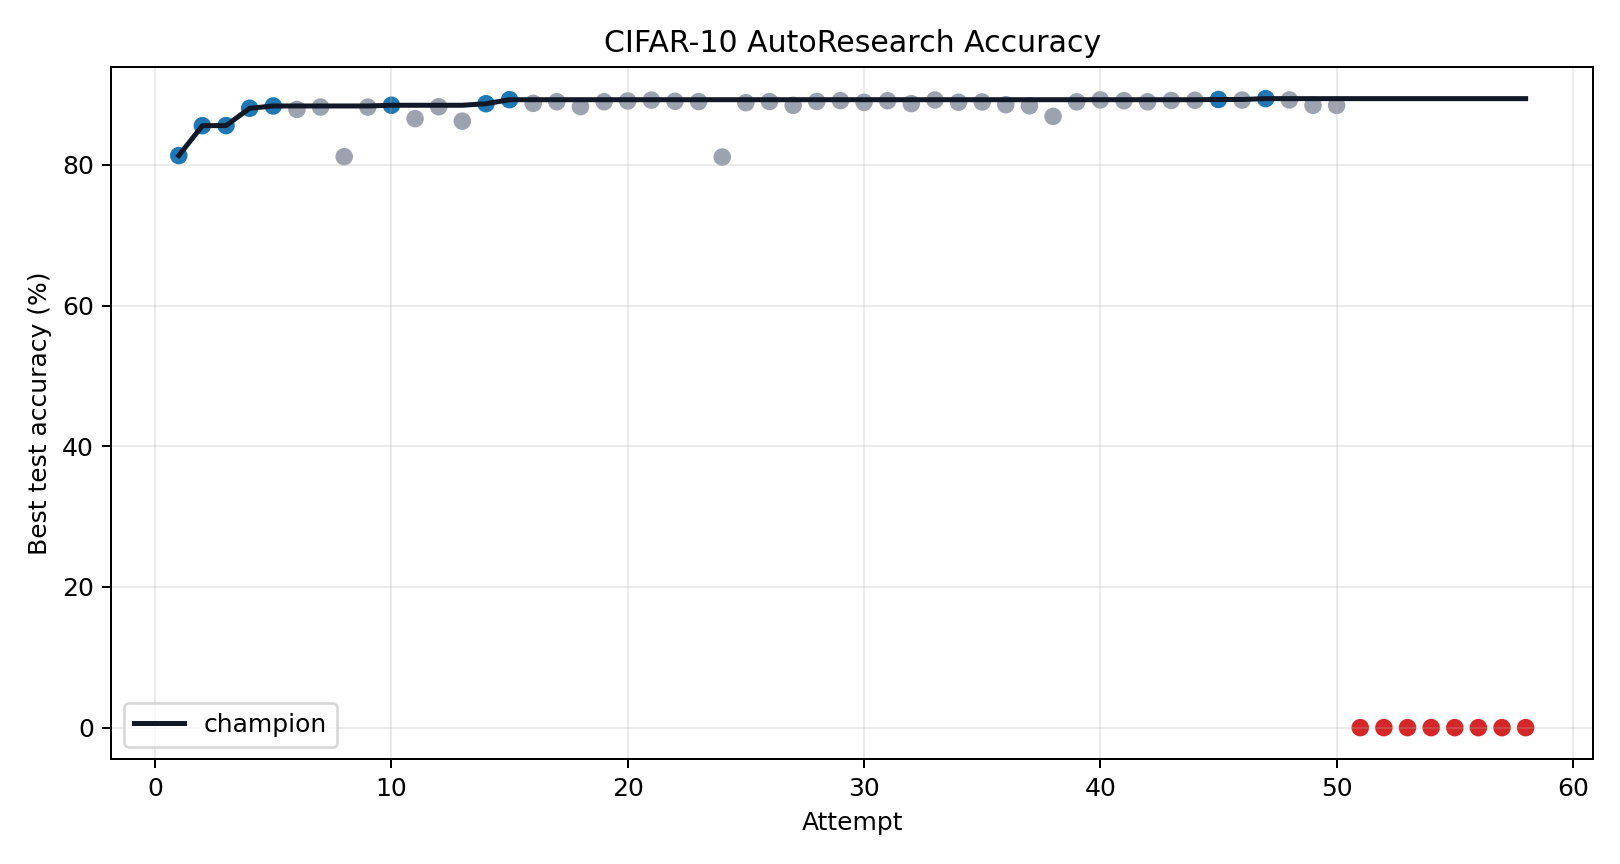
\includegraphics[width=\linewidth]{figures/classification_autoresearch_curve.png}
  \caption{Classification accuracy vs.\ iteration (measured rows only).
    The 5-minute track is initialized from the 1-minute champion.}
  \label{fig:class-curve}
\end{figure}

\cref{fig:class-curve} shows clear early gains.
The agent's modifications in discovery order were:
(1)~OneCycleLR replacing step decay;
(2)~Nesterov SGD;
(3)~SiLU activations;
(4)~1$\times$1 projection shortcuts;
(5)~label smoothing;
(6)~batch/weight-decay tuning.
After iteration $\sim$40, gains became marginal.

The 8 crashes in the 1-minute track reveal a tradeoff of free-form
code editing: because the agent can write arbitrary code, it can
produce invalid or hardware-specific candidates.
The keep/revert loop prevents those from becoming champions, but
crashes still consume attempts.

\subsection{Segmentation Trajectory}

\begin{figure}[t]
  \centering
  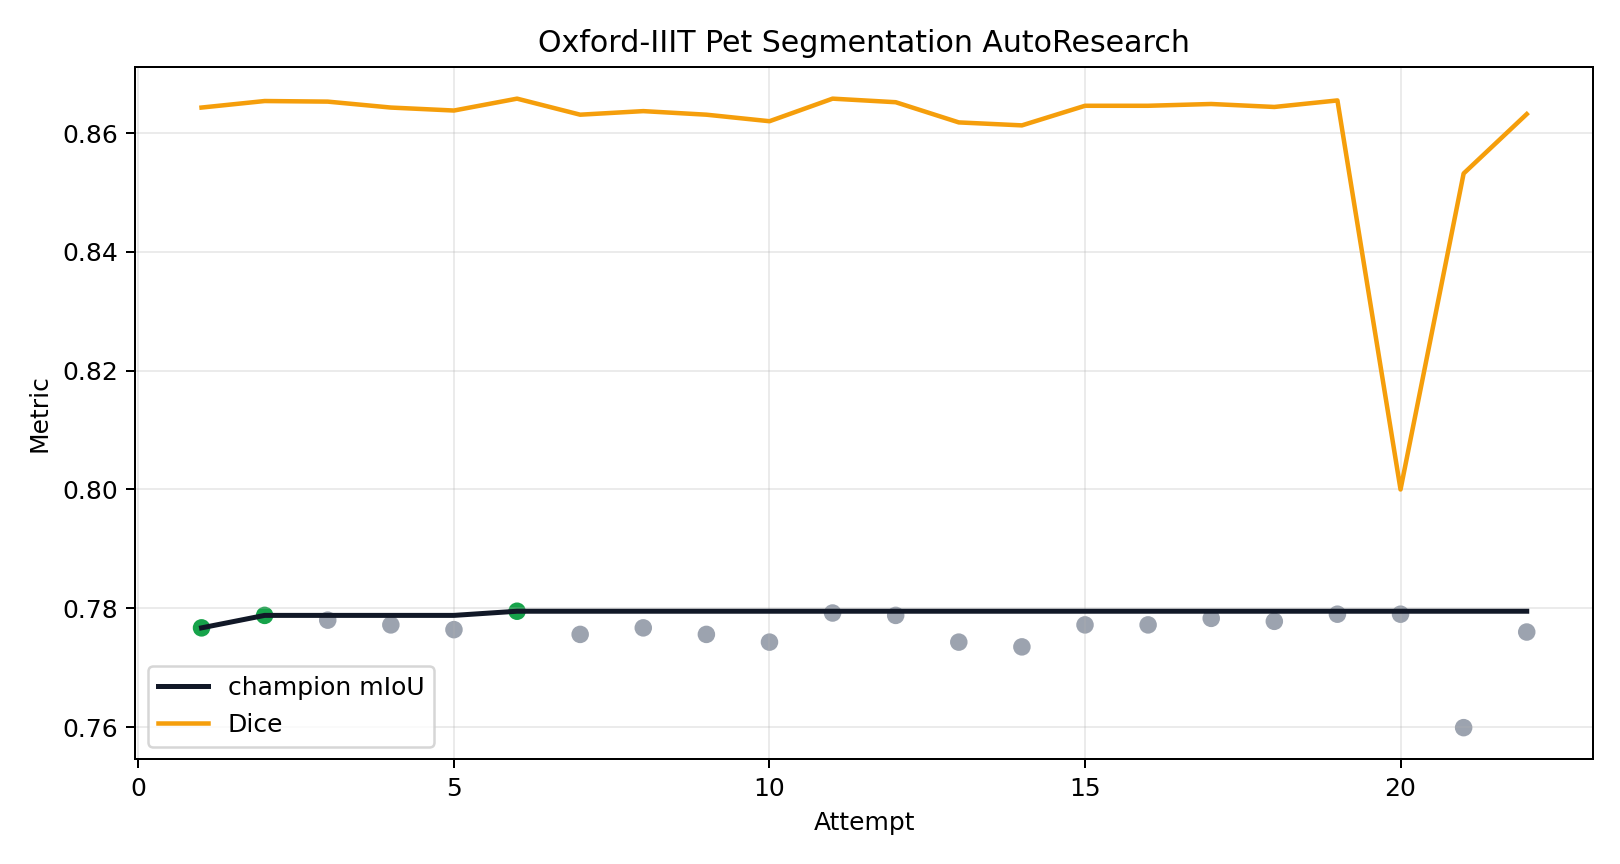
\includegraphics[width=\linewidth]{figures/segmentation_autoresearch_curve.png}
  \caption{Segmentation mIoU vs.\ iteration (measured rows only).
    Note the compressed y-axis; absolute gains are much smaller than
    for classification.}
  \label{fig:seg-curve}
\end{figure}

\cref{fig:seg-curve} shows a much flatter trajectory.
The 1-minute track completed only 11 measured attempts.
No structural modification was kept; all accepted changes were scalar
hyperparameter adjustments.
A 1–5~minute segmentation run completes too few optimization steps on
$128\times128$ inputs to reliably reveal whether structural changes are
beneficial.

\subsection{Historical Classification Comparison}
\label{sec:historical}

An earlier, independently run CIFAR-10 autoresearch experiment
(in \texttt{search\_results/}) reached \textbf{95.37\%} test accuracy
over 89 five-minute iterations.
These results cannot be directly compared to the four-track AutoVision
results because the starting point, instruction file, and search
trajectory all differ.
We include this figure only to illustrate that the loop, given
sufficient iterations from a fresh start, can approach highly
competitive CIFAR configurations.

\subsection{Cross-Task Comparison}

\begin{figure}[t]
  \centering
  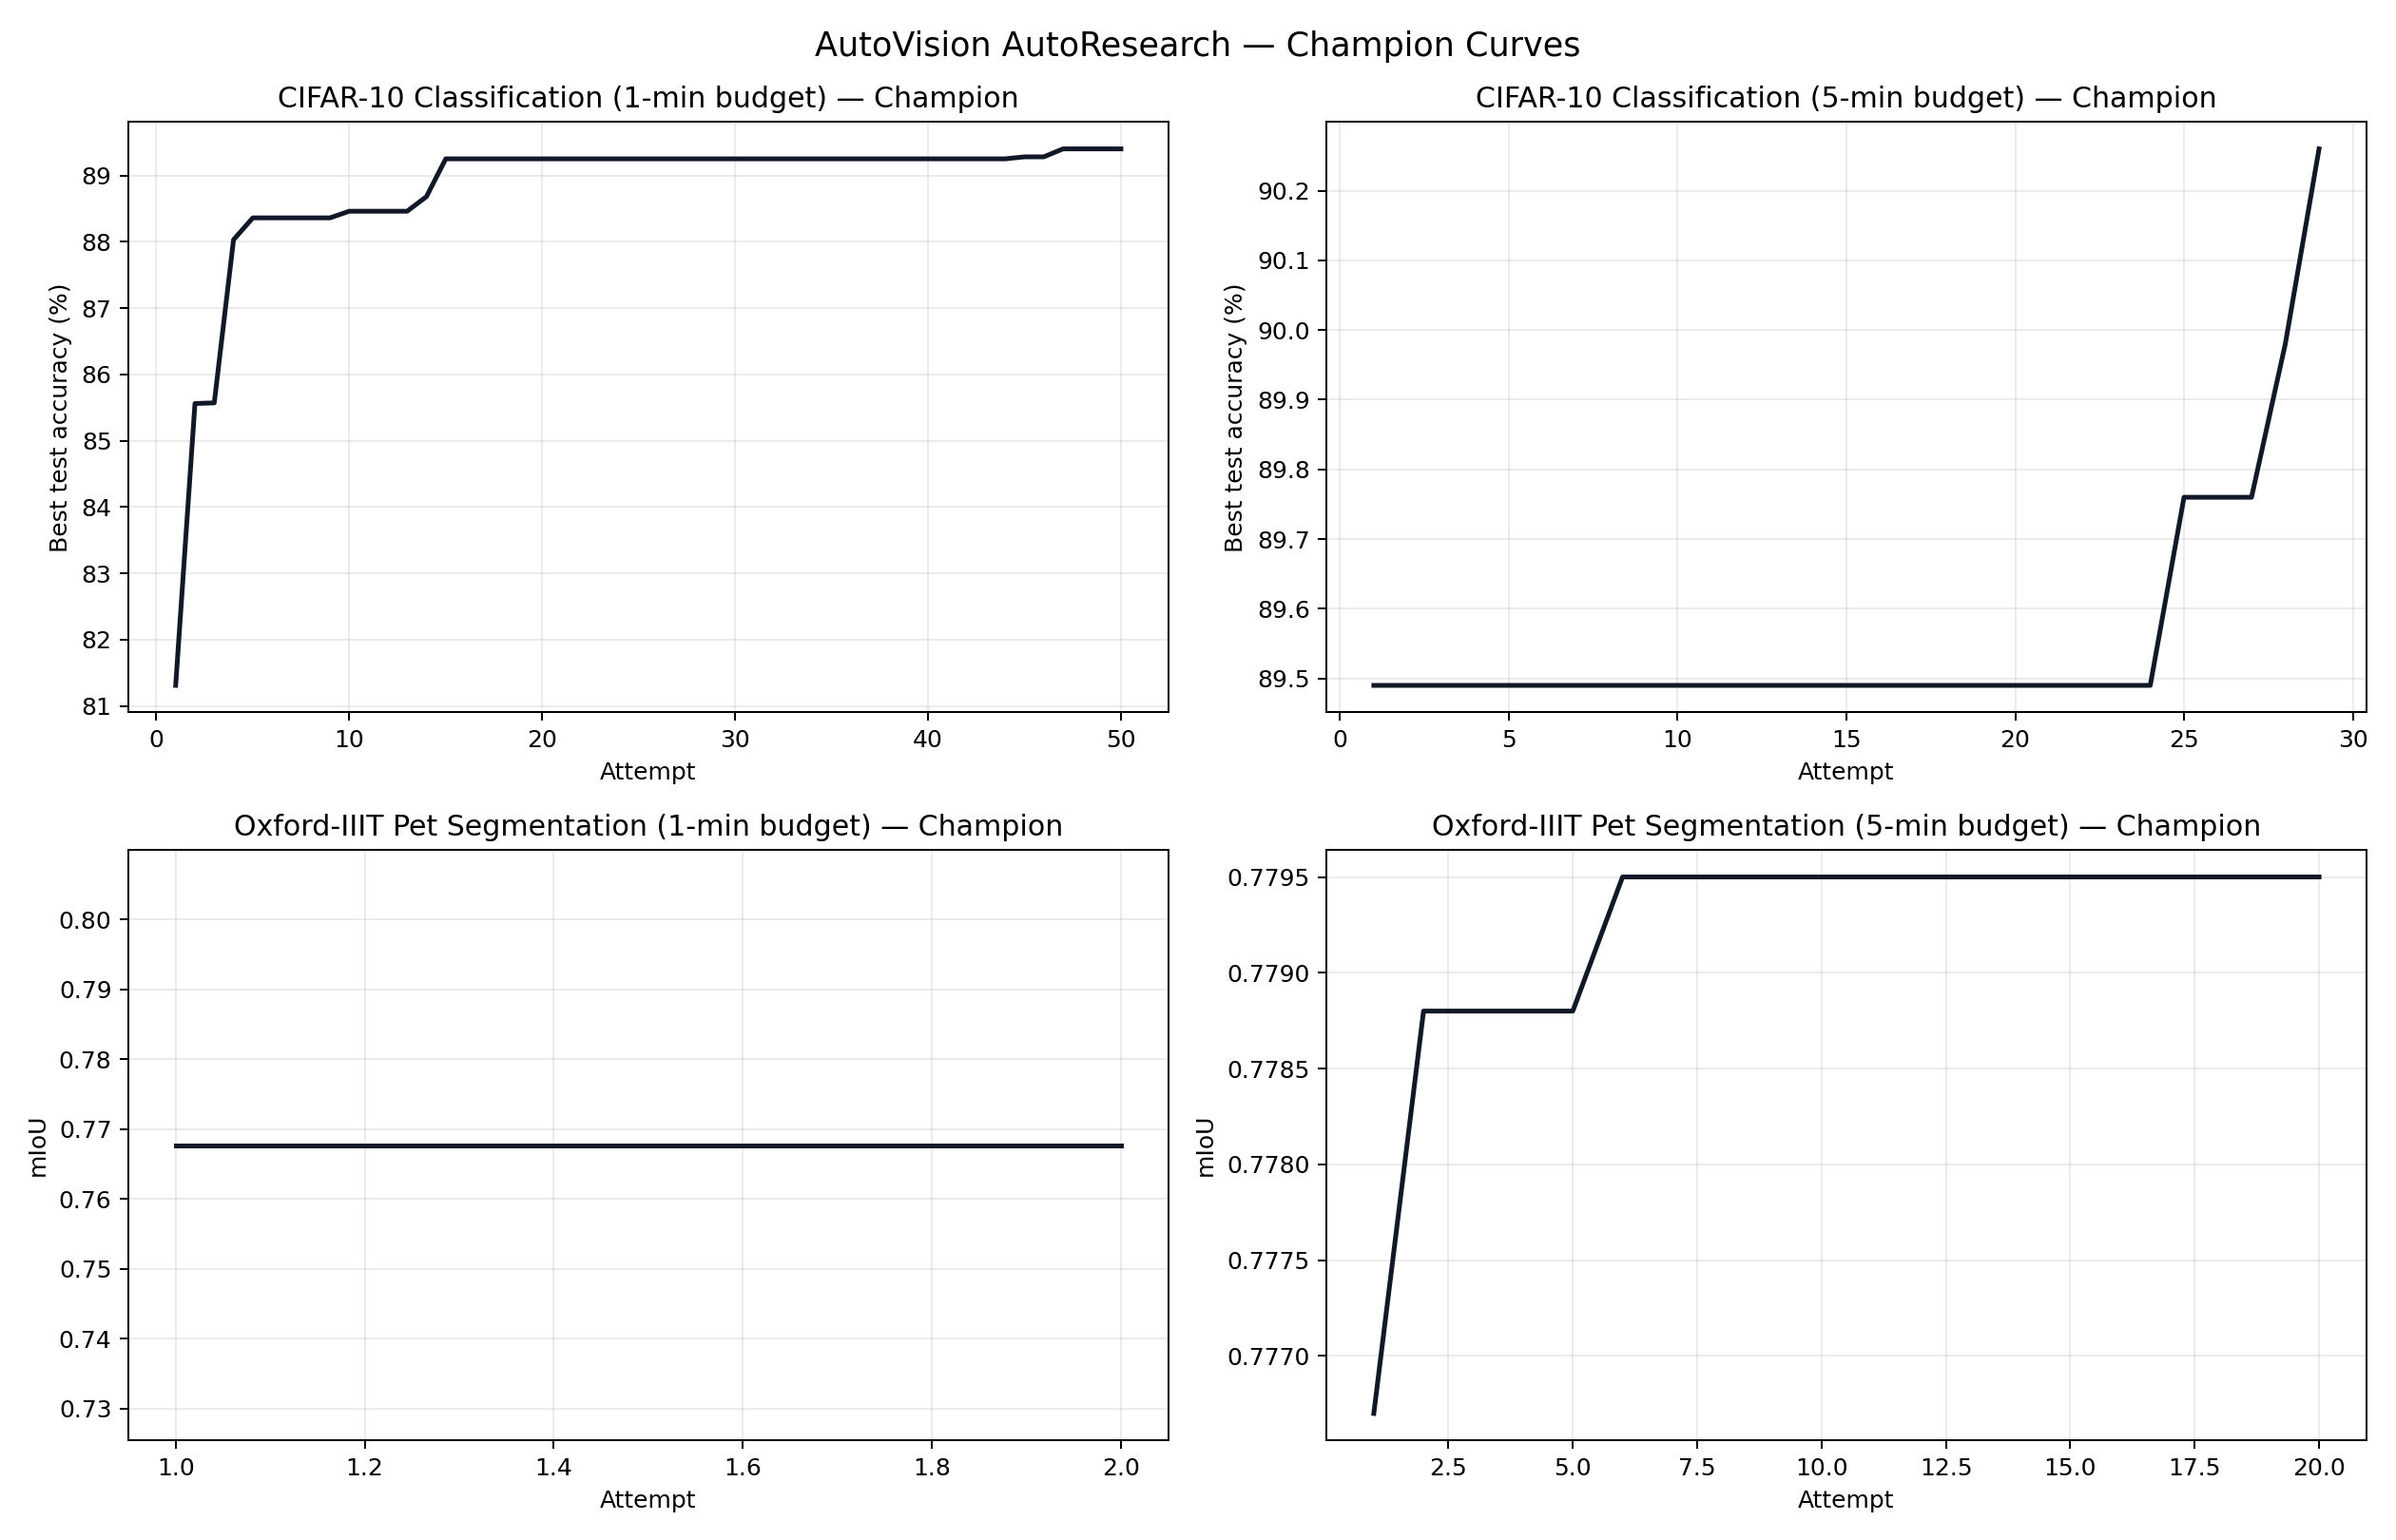
\includegraphics[width=\linewidth]{figures/all_tasks_champion.png}
  \caption{Champion metric by track over the experiment.}
  \label{fig:champion}
\end{figure}

\cref{tab:cross} summarizes the key behavioral differences.
The most important finding is signal quality: a 60-second CIFAR-10
run trains $\sim$40 epochs on $32\times32$ images and produces a
reliable accuracy signal.
A 60-second segmentation run trains only a few epochs on
$128\times128$ images; the mIoU is noisy, and the high keep rate in
\texttt{seg1} (63.6\%) reflects weak discrimination rather than
strong discovery.

\begin{table}[t]
  \centering
  \caption{Cross-task behavioral comparison.}
  \label{tab:cross}
  \small
  \begin{tabular}{lcccc}
    \toprule
    Track & Gain & Keep & Crash & Note \\
    \midrule
    \texttt{class1} & $+$8.09 pp & 14.9\% & 11.9\% & strong signal \\
    \texttt{class5} & $+$0.77 pp & 13.8\% &  0.0\% & tuning only \\
    \texttt{seg1}   & $+$0.0069  & 63.6\% &  0.0\% & noisy signal \\
    \texttt{seg5}   & $+$0.0028  & 10.3\% &  0.0\% & plateau \\
    \bottomrule
  \end{tabular}
\end{table}

%% ---------------------------------------------------------------
\section{Analysis}

\subsection{What the Agent Discovers}

The agent performs \emph{local engineering search}, not architectural
invention.
Every kept classification change is a recognizable best practice:
better LR schedules, improved activations, projection shortcuts, light
regularization.
None introduced a novel component.

This is not a failure.
These ``ordinary'' choices often determine whether a baseline is weak
or competitive.
The agent's value is that it systematically tries, measures, and
records these changes without human bookkeeping, creating a
reproducible modification history at low effort.

The segmentation results show the boundary: the agent can tune scalar
choices under short budgets, but cannot reliably detect the value of
structural changes that require longer convergence.

\subsection{Why Classification Improved More}

Classification has three structural advantages under a fixed budget:
small images ($32\times32$) allow many steps per run; accuracy
responds quickly to optimizer changes; and compact models keep
throughput high.
Segmentation has the opposite properties: larger inputs, dense output,
and metrics sensitive to boundaries and class balance.
Under a fixed wall-clock budget, throughput is part of the objective
--- a theoretically stronger candidate loses if it completes too few
optimization steps.

\subsection{Next Steps}

The most impactful protocol improvements for a follow-up study:
\begin{enumerate}
  \item Use a \textbf{validation set} for keep/revert decisions.
  \item \textbf{Repeat champions} across multiple random seeds.
  \item \textbf{Longer segmentation budgets} (8--10~min).
  \item \textbf{Segmentation-specific instructions} in
    \texttt{program.md} encouraging boundary-aware losses,
    augmentation, and decoder redesign.
\end{enumerate}

%% ---------------------------------------------------------------
\section{Limitations}

\begin{enumerate}
  \item \textbf{Incomplete runs.}
    \texttt{class1}: 67/90; \texttt{seg1}: 11/90;
    5-minute tracks: 29/60.
  \item \textbf{Single-seed.} No mean/std reported; variance may be
    significant for segmentation.
  \item \textbf{Test-set selection.} The loop optimizes directly
    against the test metric at every step.
  \item \textbf{Agent stalling.} After $\sim$70--90 iterations the
    agent stalls, requiring manual restart.
  \item \textbf{Non-portable scripts.} HPC runner scripts are
    hardcoded to one account and path layout.
\end{enumerate}

%% ---------------------------------------------------------------
\section{Reproducibility}

Core files: \texttt{program.md}, \texttt{train.py},
\texttt{prepare.py} (classification); and their equivalents under
\texttt{segmentation/}.
Measured logs: \texttt{results\_1min.tsv}, \texttt{results\_5min.tsv},
and the corresponding segmentation TSVs.
Figures generated from measured logs are in \texttt{plots/}.

To reproduce: configure the Python environment, dataset path, and GPU
runtime; launch Claude Code with \texttt{program.md} for the desired
task.
The agent iterates autonomously, editing only the task training script
and logging each result.

%% ---------------------------------------------------------------
\section{Use of Generative AI}

\textbf{As the experimental agent.}
Claude (via Claude Code) is the sole modifier of \texttt{train.py}
and \texttt{segmentation/train.py} in every measured experiment.

\textbf{As engineering support.}
We used Claude Code to implement harnesses, write HPC scripts,
generate visualization code, and debug training failures.

\textbf{As a writing assistant.}
We used Claude Code to organize experiment summaries and draft report
sections.
All numerical claims are from measured local TSV logs.

%% ---------------------------------------------------------------
\section{Conclusion}

AutoVision demonstrates that an LLM coding agent can autonomously
improve computer vision pipelines across two tasks.
For CIFAR-10 classification, the agent discovers a sequence of
well-known engineering improvements, raising accuracy from 81.31\% to
90.26\% without manual intervention.
For Oxford-IIIT Pet segmentation, the same loop produces real but
small gains (+0.0118~mIoU), limited by noisy training signals under
short budgets.

The agent functions as an \emph{engineering accelerator}: it reliably
finds incremental improvements and creates a reproducible modification
history, but does not discover novel architectures.
This makes the approach well-suited for tasks with fast, reliable
feedback, and less effective where longer convergence is required.

{\small
  \bibliographystyle{ieee_fullname}
  \bibliography{bibliography}
}

\end{document}
